\documentclass[11pt,a4j,fleqn]{jarticle}
\usepackage{amsmath,amsthm,amssymb}
\usepackage[dvipdfmx]{graphicx}

\title{課題2:レポート}
\author{著者名:村上裕亮}
\date{日付:2014.6.6}


\begin{document}

\maketitle

\section{はじめに}

このレポートでは、包絡線定理について説明し、次いで自分のコードについて説明し、工夫したところや今後の課題を説明する.

\section{包絡線定理}

\subsection{一般的な包絡線定理}
ある多変数関数($n\geq1$)$f(x_1,x_2,\cdots,x_n,t)$に対して、$t$の値をある値$\bar{t}$で固定すると、$y=f(x_1,x_2,\cdots,x_n,\bar{t})$という方程式は$n+1$次元空間の面になることが分かる.この面を$c$とする.そこで、$t$の値を1つ決めると面が1つ定まることが分かり、$t$の値を動かしてその面の通過領域の境界を$C$とすると、$C$が定まる場合がある.このときの$C$を表す関数を$F(x_1,x_2,\cdots,x_n)$とすると、
\begin{equation}
 F(x_1,x_2,\cdots,x_n)=\max_t f(x_1,x_2,\cdots,x_n,t)\label{eq:max}
\end{equation}
ないし、
\begin{equation}
 F(x_1,x_2,\cdots,x_n)=\min_t f(x_1,x_2,\cdots,x_n,t)\label{eq:min}
\end{equation}
となるはずだ.

また、このとき、F上の点を1点とり、その点を$(x_1^*,x_2^*,\cdots,x_n^*)$とすると、この点に対応する$t$は\eqref{eq:max}や\eqref{eq:min}を解いた最大化(最小化)問題の解になるので一意に定まることが分かる.その解を$\bar{t}$とおくと、面$C$と面$c$は$(x_1^*,x_2^*,\cdots,x_n^*,\bar{t})$で接することが分かる.したがって、面$C$の点$(x_1^*,x_2^*,\cdots,x_n^*)$での接面を求めたければ、面$c$の点$(x_1^*,x_2^*,\cdots,x_n^*,\bar{t})$での接面を求めれば良いと分かる.$F$上の全ての点で同じことが言えるので、全ての$i(1\leq i\leq n)$について以下が成立する.
\begin{equation}
 \frac{\partial}{\partial x_i}F(x_1,x_2,\cdots,x_n)=\frac{\partial f}{\partial x_i}(x_1,x_2,\cdots,x_n,\bar{t})\label{eq:square}
\end{equation}
ここで、$F(x_1,x_2,\cdots,x_n)=f(x_1,x_2,\cdots,x_n,\bar{t})$だから、\eqref{eq:square}は
\begin{equation}
 \frac{\partial}{\partial x_i}f(x_1,x_2,\cdots,x_n,\bar{t})=\frac{\partial f}{\partial x_i}(x_1,x_2,\cdots,x_n,\bar{t})\label{eq:square-2}
\end{equation}
と変形できる.\eqref{eq:square-2}の主張は、接点(=最大化問題を解いた解)であれば、代入してから微分しても、微分してから代入しても結果は変わらないというところにあり、これが包絡線定理の主張となる(尾山・安田\cite{OyamaYasuda11}).

\subsection{具体例}

$n=1$の場合で、多変数関数を
\begin{equation}
 f(x,t)=xt-t^2 \label{eq:def}
\end{equation}
とする.$t$を実数全体で動かしたときの包絡線を求めると、\eqref{eq:def}は$t$について2次関数なので、
\begin{equation*}
 f(x,t)=-\left(t-\frac{x}{2}\right)^2+\frac{x^2}{4}
\end{equation*}
となるので、
\begin{equation*}
 F(x)=\max_t f(x,t)=\frac{x^2}{4}
\end{equation*}
と分かる.このことをPythonに図示させたのが以下の図\ref{fig:1}や図\ref{fig:2}だ.
\begin{figure}[htb]
 \centering
 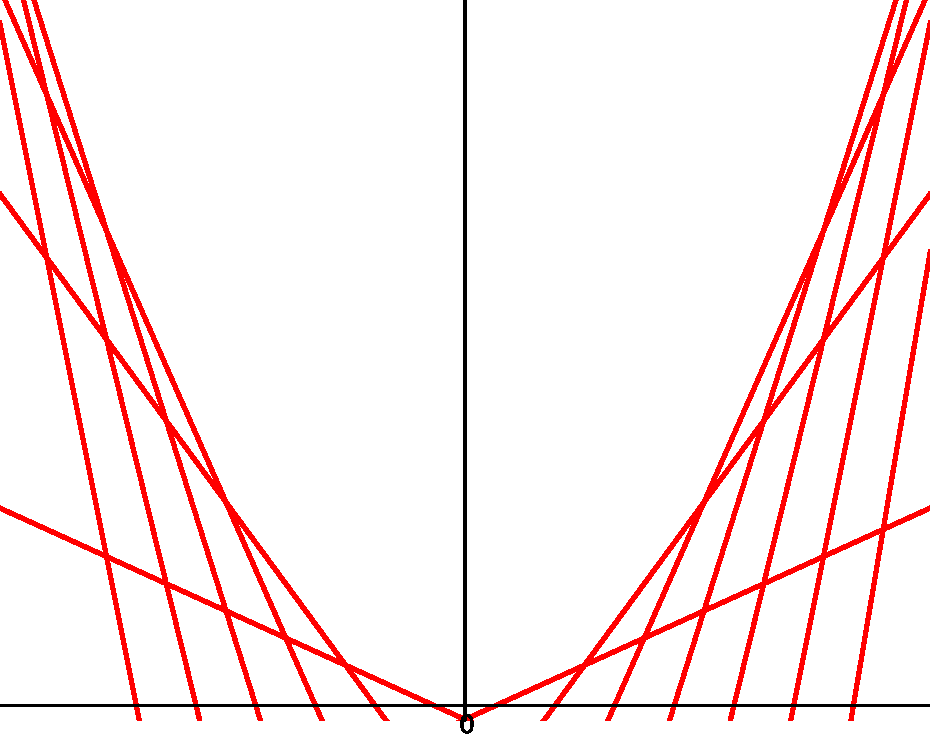
\includegraphics[scale=0.4]{envelope0.pdf}
 \caption{包絡線(1)}
 \label{fig:1}
 \centering
 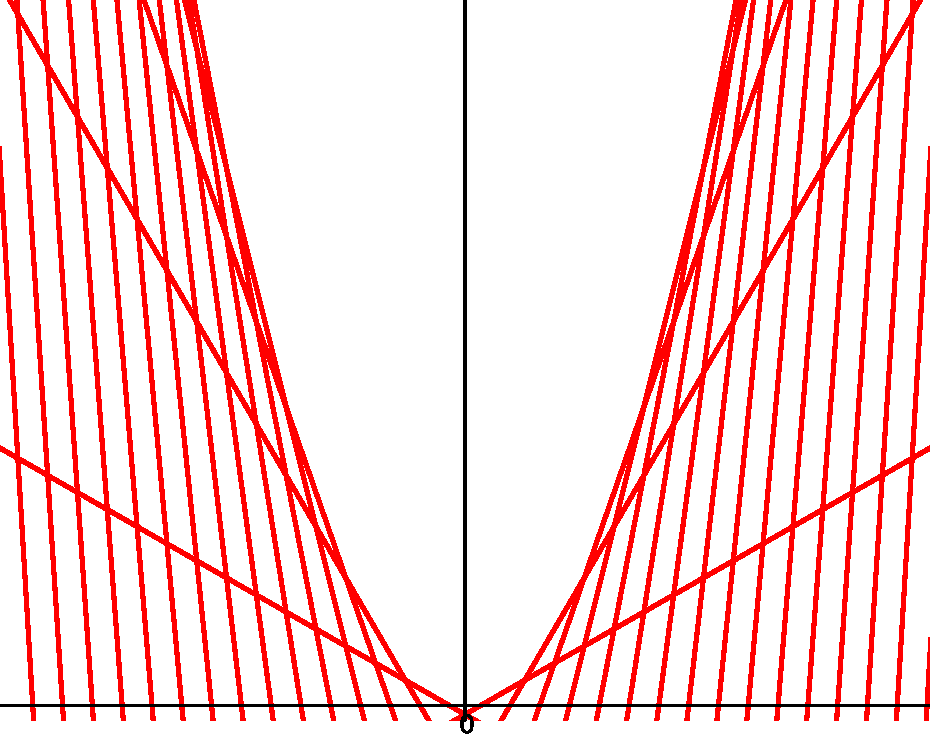
\includegraphics[scale=0.4]{envelope1.pdf}
 \caption{包絡線(2)}
 \label{fig:2}
\end{figure}

これらの形を見ると、放物線の形が見えることが分かる.

\section{Pythonプログラム}

\subsection{用いたコード}

今回表示するのに用いたPythonのコードは以下だ.
\begin{quote}
\begin{verbatim}
from mpl_toolkits.axes_grid.axislines import SubplotZero
import matplotlib.pyplot as plt
import numpy as np
import pylab as pl

FIGNUM = 0

if FIGNUM == 0:
    n = 13
    area = 1
if FIGNUM == 1:
    n = 31
    area = 1.5


def f(x,a):
    return area*(-x**2+a*x)

def subplots():
    
    fig = plt.figure(1)
    ax = SubplotZero(fig, 111)
    fig.add_subplot(ax)

    for direction in ["xzero", "yzero"]:
        ax.axis[direction].set_axisline_style("-|>")
        ax.axis[direction].set_visible(True)

    for direction in ["left", "right", "bottom", "top"]:
        ax.axis[direction].set_visible(False)

    return fig, ax

fig, ax = subplots() 

plt.axis([-n**0.8, n**0.8, -n*0.02, n])

plt.xticks([0])
plt.yticks([])

a = np.linspace(-2*n, 2*n, 100*n)

for x in range(n):
    y = f(x-n/2+0.5, a)
    ax.plot(a, y, 'r-', linewidth=2)
plt.savefig('envelope' + str(FIGNUM) + '.png', 
transparent=True, bbox_inches='tight', pad_inches=0)
plt.savefig('envelope' + str(FIGNUM) + '.pdf', 
bbox_inches='tight', pad_inches=0)
plt.show()
\end{verbatim}
\end{quote}

以降、このコードについての説明を施す.

\begin{quote}
\begin{verbatim}
from mpl_toolkits.axes_grid.axislines import SubplotZero
import matplotlib.pyplot as plt
import numpy as np
import pylab as pl
\end{verbatim}
\end{quote}
では、必要なモジュールをPythonに読み込んだ.
\begin{quote}
\begin{verbatim}
FIGNUM = 0

if FIGNUM == 0:
    n = 13
    area = 1
if FIGNUM == 1:
    n = 31
    area = 1.5
\end{verbatim}
\end{quote}
では、\verb|FIGNUM|を\verb|0|と\verb|1|で切り替えることで、2種類のパラメータの切り替えを行った.ここで、\verb|n|は直線の本数、\verb|area|はその密度(値が大きいほど疎、小さいほど密)を表している.

\begin{quote}
\begin{verbatim}
def f(x,a):  
    return area*(-x**2+a*x)
\end{verbatim}
\end{quote}
では、今回用いる関数を定義した.ここで式全体に\verb|area|がかかっているのは、密度を変化させるためだ.

\begin{quote}
\begin{verbatim}
def subplots():
    
    fig = plt.figure(1)
    ax = SubplotZero(fig, 111)
    fig.add_subplot(ax)

    for direction in ["xzero", "yzero"]:
        ax.axis[direction].set_axisline_style("-|>")
        ax.axis[direction].set_visible(True)

    for direction in ["left", "right", "bottom", "top"]: 
        ax.axis[direction].set_visible(False)

    return fig, ax

fig, ax = subplots()
\end{verbatim}
\end{quote}
では、グラフの軸などを変更した(ヒントはWeb\cite{web}から得た).具体的には、軸を表示させ、デフォルトでは周囲に値が表示されるがそれを消した.

\begin{quote}
\begin{verbatim}
plt.axis([-n**0.8, n**0.8, -n*0.02, n])

plt.xticks([0])
plt.yticks([])
\end{verbatim}
\end{quote}
では、グラフの表示される領域と、軸上に表示させる数値を入力している.ここで、グラフの表示領域に\verb|n|が含まれているのは、直線の本数に応じて表示領域を変化させるためだ.横軸上に0をプロットし、それ以外の数字は表示させていない.

\begin{quote}
\begin{verbatim}
a = np.linspace(-2*n, 2*n, 100*n)
\end{verbatim}
\end{quote}
では、\verb|a|で直線の幅を設定した(ここでは\verb|-2*n|から\verb|2*n|).

\begin{quote}
\begin{verbatim}
for x in range(n):
    y = f(x-n/2+0.5, a)
    ax.plot(a, y, 'r-', linewidth=2)
\end{verbatim}
\end{quote}
では、\verb|x|をパラメーターにfor文で繰り返し直線を引いた.\verb|ax.plot|は、\verb|a|の間隔ごとに\verb|y|をとり、その間は直線で補完して線を描く指示をしている.

\begin{quote}
\begin{verbatim}
plt.savefig('envelope' + str(FIGNUM) + '.png', 
transparent=True, bbox_inches='tight', pad_inches=0)
plt.savefig('envelope' + str(FIGNUM) + '.pdf', 
bbox_inches='tight', pad_inches=0)
plt.show()
\end{verbatim}
\end{quote}
では、完成した図をpng形式とpdf形式のファイルにそれぞれ保存し、最後にその図を表示させている.

\subsection{このコードの課題}
グラフの描画範囲は今回は恣意的に\verb|plt.axis([-n**0.8, n**0.8, -n*0.02, n])|としたが、包絡線の形によって描画範囲はその都度変えなければならず、多変数方程式の形が変わると対応できないことになってしまう.望ましいのは包絡線全体が映り、かつ、それ以外の部分はあまり映らないことで、包絡線と直線(場合によっては曲線)の接点の座標を取得して、その範囲というように設定するのが本来は望ましいと思われる.

\begin{thebibliography}{0}
\bibitem{OyamaYasuda11}
尾山大輔・安田洋祐「経済学で出る包絡線定理」『経済セミナー』2011年10・11月号.
\bibitem{web}
http://matplotlib.org/examples/axes\_grid/demo\_axisline\_style.html
\end{thebibliography}



\end{document}